%&latex
%
\providecommand{\main}{../..}
\documentclass[../../main.tex]{subfiles}

\begin{document}

\subsection{Variation: infection from outside}
\lesson{36}{01/06/20}
Suppose that healthy individuals can become infected with a constant rate $h \neq 0$ \textit{independent} on the state of their neighbours (i.e. they are infected from an \q{external field}). The new rate for the transition $n \to n+1$ becomes:
\begin{align*}
    b_h(n) = b(n) + \underbrace{(N-m)}_{\mathclap{\text{N. of healthy}}}  h
\end{align*} 
The evolution of the average number of infected is then:
\begin{align*}
    \dv{t} \langle n \rangle:t = \langle b_h(n) - d(n) \rangle_t = \langle b(n) - d(n) \rangle_t + h(N - \langle n \rangle_t)
\end{align*}
And (\ref{eqn:contact-evo3}) gains an additional term:
\begin{align*}
    \dv{\rho}{t} = (\lambda - 1) \rho - \lambda \rho^2 + h(1-\rho)
\end{align*}
In this case, $\rho^* = 0$ is not a stationary state anymore. Instead, we have a unique stationary state:
\begin{align*}
    \bar{\rho} = \frac{1}{2 \lambda} [\lambda - h - 1 + \sqrt{(\lambda - h - 1)^2 + 4 \lambda h}]
\end{align*}

At the critical point, $\lambda = 1$, with $h > 0$ and small:
\begin{align*}
    \bar{\rho} = \frac{1}{2} [ - h + \sqrt{h^2 + 4h}]  = h^{\textcolor{Red}{1/2}} ( 1 + O(h) ) \sim h^{\textcolor{Red}{1/\delta}} \qquad \textcolor{Red}{\delta} = 2
\end{align*}
which is again a power-law, similar to the one we found in the mean field IM (where, however, $\delta = 3$).

\subsection{Spatial effects}
If we want to study \textit{spatial effects}, we need to make nodes only \textit{locally} connected.

Then, for each node $x$:
\begin{itemize}
    \item The transition $1 \to 0$ (recovery) happens with a fixed rate of $w_{x}^-(\sigma) = 1$.
    \item The transition $0 \to 1$ (infection) happens with a rate proportional to $\lambda$ and the fraction of infected nearest neighbours:
    \begin{align*}
        w_{x}^+(\sigma) = \frac{\lambda}{2d} \> \> \> \sum_{\mathclap{y \in \langle x,y \rangle}} \sigma_y
    \end{align*} 
\end{itemize}
We can \textit{merge} both cases as follows:
\begin{align}\label{eqn:contact-transition-rate}
    w_x(\sigma) = \textcolor{Red}{\sigma_x} \cdot 1 + \textcolor{Red}{(1-\sigma_x)} \cdot \frac{\lambda}{2d} \>\>\> \sum_{\mathclap{y \in \langle x,y \rangle}}  \sigma_y
\end{align} 
Here $w_x(\sigma)$ is the rate of $x$ \textit{flipping} state. If $\sigma_x = 0$ (healthy), then only the second term will matter, and if $\sigma_x = 1$ (infected) only the first one is non-zero.

\medskip

As we did in studying the Ising Model dynamics, we define the state $\bm{\sigma^{(x)}}$ as equal to $\bm{\sigma}$ with the $x$-th state flipped:
\begin{align*}
    \sigma_y^{(x)} = \begin{cases}
        \sigma_y & y \neq x\\
        1 - \sigma_x & y = x
    \end{cases} \qquad y = 1,\dots,N
\end{align*}

With this notation we can write the system's Master Equation as follows:
\begin{align}\label{eqn:contact-ME2}
    \dot{\mathbb{P}}(\bm{\sigma}; t) = \sum_{x} [w_x (\bm{\sigma^{(x)}}) \mathbb{P}(\bm{\sigma^{(x)}}; t) - w_x(\bm{\sigma}) \mathbb{P}(\bm{\sigma}; t)]
\end{align}

The evolution of the fraction of infected can be computed as:
\begin{align*}
    \dv{t} \langle \sigma_z \rangle_t &= \sum_{\{\bm{\sigma}\}} \dot{\mathbb{P}}(\bm{\sigma},t) \sigma_z \underset{\mathclap{(\ref{eqn:contact-ME2})}}{=}  
    \sum_x \sum_{\{\bm{\sigma}\}} \sigma_z [w_x(\bm{\sigma^{(x)}}) \mathbb{P}(\bm{\sigma^{(x)}};t) - w_x(\bm{\sigma}) \mathbb{P}(\bm{\sigma};t)] =\\
    \intertext{Exchanging $\bm{\sigma} \leftrightarrow \bm{\sigma^{(x)}}$ in the first sum, we can \textit{merge} the two terms:}
    &= \sum_{\{\bm{\sigma}\}} \mathbb{P}(\bm{\sigma}; t) \sum_x w_x(\bm{\sigma}) \underbrace{(\sigma_z^{(x)} - \sigma_z)}_{\mathclap{= 0 \text{ if $x \neq z$}}} = \langle w_z(\bm{\sigma}) (1-2\sigma_z) \rangle_t =\\
    &\underset{\mathclap{(\ref{eqn:contact-transition-rate})}}{=} \langle \Big(\sigma_z + \frac{\lambda}{2d} (1-\sigma_z) \sum_{\mathclap{y \in \langle x,y \rangle}} \sigma_y  \Big)(1 - 2 \sigma_z) \rangle_t =\\
    &\underset{\mathclap{\sigma_z^2 = \sigma_z}}{=} - \langle \sigma_z \rangle_t + \frac{\lambda}{2d} \langle (1-\sigma_z) \sum_{\mathclap{y \in \langle x,y \rangle}} \sigma_y \rangle_t 
\end{align*}
Using the definition of a discrete laplacian (\ref{eqn:discrete-laplacian}, pag. \pageref{eqn:discrete-laplacian}) we have:
\begin{align*}
    \sum_{\mathclap{y \in \langle x,y \rangle}} \sigma_y = \bigtriangleup_z \sigma_z + 2 d \sigma_z
\end{align*}
And we approximate by \textit{factorizing} the average: 
\begin{align*}
    \dv{t} \langle \sigma_z \rangle \approx - \langle \sigma_z \rangle_t + \frac{\lambda}{2d} \langle 1 - \sigma_z \rangle_t (\bigtriangleup_z \langle \sigma_z \rangle_t + 2d \langle \sigma_z \rangle_t)
\end{align*}
Denoting $\langle \sigma_z \rangle_t \equiv \rho(z;t)$:
\begin{align}\nonumber
    \dot{\rho} &= - \rho + \frac{\lambda}{2d} \left[(1-\rho) \nabla^2 \rho + 2d (1-\rho)\rho\right] \\
    &= (\lambda - 1) \rho - \lambda \rho^2 + \frac{\lambda}{2d} (1 - \rho) \nabla^2 \rho \label{eqn:contact-evo4} 
\end{align}
Comparing with the mean field equation (\ref{eqn:contact-evo3}), the only additional term is the one with the laplacian, which gives the equation a \textit{diffusion}-like nature. Note that the diffusion rate is regulated by $(1-\rho)$, meaning it is constant when $\rho \approx 0$, and vanishes when $\rho \to 1$, since when almost everyone is infected, the number of pairs of neighbouring susceptible-infected nodes are few.

\medskip

Again we have two cases:
\begin{itemize}
    \item If $\Delta = \lambda -1 < 0$, then the system will tend towards the absorbing state $\rho^* = 0$. Let's denote $\rho \equiv \rho_-$ and study the dynamics near stationarity, i.e. when $\rho_- \approx 0$. Equation (\ref{eqn:contact-evo4}) becomes:
    \begin{align*}
        \dot{\rho}_- = \Delta \cdot \rho_- + D_- \nabla^2 \rho_- \qquad D_- \equiv \frac{\lambda}{2d} 
    \end{align*}
    \item If $\Delta = \lambda -1 > 0$, the stationary state will be $\bar{\rho} = +\Delta/\lambda$. Let's denote $\rho(x;t) - \bar{\rho} \equiv \rho_+(x;t)$, equation (\ref{eqn:contact-evo4}) becomes:
    \item \begin{align*}
        \dot{\rho}_+ &= - \Delta \cdot \rho_+ - \lambda \rho_+^2 + D_+(1-\bar{\rho} - \rho_+) \nabla^2 \rho_+ =\\
        &\approx -\Delta \cdot \rho_+ + D_+ \nabla^2 \rho_+ \qquad D_+ \equiv D_- (1  - \bar{\rho})
    \end{align*}%TODO Do computations
\end{itemize}

Thus in both cases we have to solve an equation of the form:
\begin{align*}
    \dot{\varphi}(\bm{x},t) = - a \varphi + b \nabla^2 \varphi \qquad a,\, b > 0
\end{align*}%TODO Fix vectors

To solve it, we use the Fourier transform:
\begin{align*}
    \tilde{\varphi}(\bm{p}, t) = \int_{\mathbb{R}^d} e^{i \bm{p} \cdot \bm{x}} \varphi(\bm{x}, t) \dd[d]{\bm{x}} \qquad \varphi(\bm{x},t) = \int_{\mathbb{R}^d} e^{-i \bm{p}\cdot \bm{x}} \tilde{\varphi}(\bm{p},t) \frac{\dd[d]{\bm{p}}}{(2 \pi)^d} 
\end{align*}
Transforming both sides we get:
\begin{align*}
    \dot{\tilde{\varphi}}(\bm{p}, t) = - (a + b \norm{\bm{p}}^2 ) \tilde{\varphi}(\bm{p}, t)
\end{align*}
which can be immediately integrated:
\begin{align*}
    \tilde{\varphi}(\bm{p}, t) = e^{-(a+b\norm{\bm{p}}^2)t} \tilde{\varphi}(\bm{p},0) = e^{-(a + b\norm{\bm{p}}^2)t} \int_{\mathbb{R}^d} \dd[d]{\bm{x'}} e^{i \bm{p} \cdot \bm{x'}} \varphi(\bm{x'},0)
\end{align*}
And inverting the transform leads to:
\begin{align*}
    \varphi(\bm{x}, t) &= e^{-at} \int_{\mathbb{R}^d} \dd[d]{\bm{x'}} \int_{\mathbb{R}^d} \frac{\dd[d]{\bm{p}}}{(2\pi)^d} e^{-i \bm{p} \cdot (\bm{x} - \bm{x'}) - (a + \norm{\bm{p}}^2 b)t} \varphi(\bm{x'}, 0) =\\
    &= e^{-a t} \int_{\mathbb{R}^d} \frac{\dd[d]{\bm{x'}}}{(4 \pi b t)^{d/2}} \exp\left(-\frac{\norm{\bm{x} - \bm{x'}}^2}{4bt} \right) \varphi(\bm{x'},0)
\end{align*}

Adapting to the two cases:
\begin{align*}
    \rho_{\pm}(\bm{x}, t) = \int_{\mathbb{R}^d} \dd[d]{\bm{x'}} \underbrace{\frac{\displaystyle e^{-|\Delta|t} \exp\left(-\frac{\norm{\bm{x} - \bm{x'}}^2}{4 D_\pm t} \right)}{(4 \pi D_\pm t)^{d/2}}}_{G_\pm(\bm{x} - \bm{x'},t)}   \rho_{\pm}(\bm{x'},0)
\end{align*}
where $G_\pm(\bm{x}-\bm{x'};t)$ is the \textbf{propagator} that makes the initial condition \q{evolve}.

\medskip

If we choose an initial condition with only one infected individual, i.e. $\rho_{\pm} (\bm{x'}, 0) = \delta^d(\bm{x'})$, the epidemic will spread, but also dampen over time (the area below the curve vanishes):
\begin{align}\label{eqn:contact-sol}
    \rho_{\pm}(\bm{x},t) = G_{\pm}(\bm{x},t) = \frac{e^{-|\Delta|t} \exp\left(-\frac{\norm{\bm{x}}^2}{4 D_{\pm} t} \right)}{(4 \pi D_{\pm} t)^{d/2}} 
\end{align}

\begin{figure}[H]
    \centering
    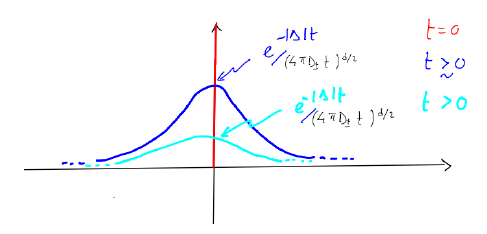
\includegraphics[width=0.8\textwidth]{\main/Images/contact-evo.png}
    \caption{Example of evolution for a system with a single initial infected individual.}
    \label{fig:contact-evo}
\end{figure}

A simulation in $d=1$ of the contact process for different values of $\lambda$ is shown in fig. \ref{fig:contact-simulation}.

\begin{figure}[H]
    \centering
    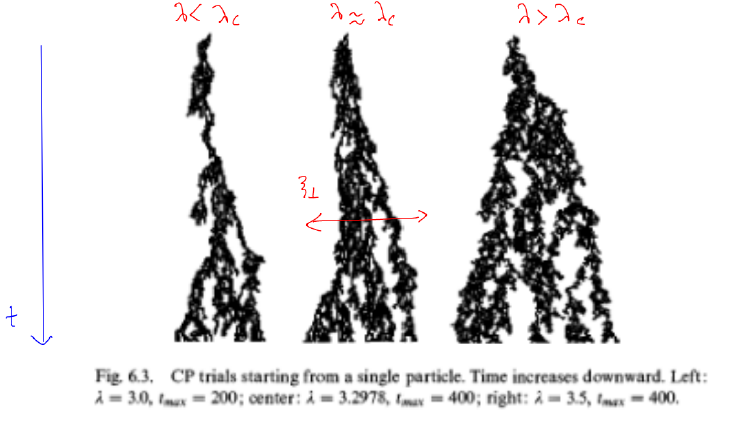
\includegraphics[width=0.8\textwidth]{\main/Images/contact-simulation.png}
    \caption{Examples of evolution}
    \label{fig:contact-simulation}
\end{figure}

Let $\rho(\bm{r},t)$ be the probability that a node at position $\bm{r}$ is infected at time $t$, given the fact that there was an infected at $\bm{r}=0$ at $t=0$:
\begin{align*}
    \rho(\bm{r},t) = \langle \delta_{\sigma_{\bm{r}}(t),1} \rangle = \langle \sigma_{\bm{r}} \rangle_t
\end{align*}
It can be shown \textit{numerically} that $\rho(\bm{r},t)$, near criticality $\lambda \lesssim \lambda_c$, $\Delta = \lambda - \lambda_c \approx 0^-$, scales according to a power-law:
\begin{align*}
    \rho(\bm{r},t|\Delta) = t^{-\psi} F\left(\frac{r}{t^{z/2}, t |\Delta|^{v_\parallel}} \right)
\end{align*}  
where $F$ is a function of two (non-trivial) \textit{dimensionless} variables, where $\tau \propto |\Delta|^{-v_\parallel} \equiv \xi_\parallel$ is a characteristic critical timescale, and $\xi_\perp \propto \tau^{z/2} \propto |\Delta|^{-v_\perp}$ is a characteristic critical spatial scale, with $v_\perp = z/(2 v_\parallel)$. %Parallel and perpendicular refer to the directions in the graph of fig:contact-simulation

\medskip

When $\lambda < \lambda_c$, equation (\ref{eqn:contact-sol}) gives:
\begin{align}
    \rho_{\pm}(\bm{r},t) = \frac{e^{-|\Delta|t} \exp\left(-\frac{\norm{\bm{r}}^2}{4 D_{\pm} t} \right)}{(4 \pi D_{\pm} t)^{d/2}} 
\end{align}
and so we find the \textit{mean field} values of the exponenents $\psi = d/2$, $v_\parallel = 1$, $z=1$ and $v_\perp = 1/2$.

\begin{exo}[MaxEnt and Networks]
    Let $G$ be a network (i.e. a graph), with a certain number of \textit{vertices} connected by \textit{edges}.
    Suppose we have measured some property of $G$, e.g. the number of edges $m(G)$, and we want to find the most unbiased distribution of networks $\mathbb{P}(G)$ that is compatible with our observations.

    Explicitly, suppose that we know the average of $x$:
    \begin{align}\label{eqn:mean-constraint}
        \langle x \rangle = \sum_G \mathbb{P}(G) x(G)
    \end{align}
    Then as a consequence of the MaxEnt principle, we choose $\mathbb{P}(G)$ such that its entropy $S(G)$ is maximum:
    \begin{align*}
        S(G) = - \sum_G \mathbb{P}(G) \ln \mathbb{P}(G)
    \end{align*}
    with $\mathbb{P}(G)$ subject to the constraint (\ref{eqn:mean-constraint}) and the normalization condition:
    \begin{align*}
        \sum_G \mathbb{P}(G) \overset{!}{=}  1
    \end{align*}
    Using the method of Lagrange multipliers leads to:
    \begin{align*}
        \pdv{\mathbb{P}(G)} \left[-\sum_G \mathbb{P}(G) \ln \mathbb{P}(G) - \theta \sum_G x(G) \mathbb{P}(G) - \alpha \sum_G \mathbb{P}(G)\right] \overset{!}{=}  0
    \end{align*}
    with solution (as we've already seen):
    \begin{align}\label{eqn:graph-maxent-sol}
        \mathbb{P}(G) = \frac{1}{Z(\theta)} e^{-\theta x(G)} \qquad Z(\theta) = e^{\alpha + 1} = \sum_G e^{-\theta x(G)} 
    \end{align}

    As an example, let $x(G) = m(G)$ be the number of edges. For each pair of vertices $(i,j) \in G$ we define a binary variable:
    \begin{align*}
        \sigma_{ij} = \begin{cases}
            1 & \text{if $i$ is connected to $j$}\\
            0 & \text{otherwise}
        \end{cases}
    \end{align*} 
    The set of all $\sigma_{ij}$ \textit{defines} the entire graph $G = \{\sigma_{ij} \colon i \neq j; i, j = 1,\dots, n\}$. In particular, the number of edges can be written as:
    \begin{align*}
        m(G) \equiv m(\bm{\sigma}) = \sum_{i < j} \sigma_{ij}
    \end{align*}
    Substituting in (\ref{eqn:graph-maxent-sol}) leads to:
    \begin{align*}
        \mathbb{P}(G) &\equiv \mathbb{P}(\bm{\sigma}) = \frac{\exp\left(-\theta \sum_{i < j} \sigma_{ij}\right)}{Z(\theta)} \\
        Z(\theta) &=  \sum_{\{\bm{\sigma}\}} \exp\left(-\theta \sum_{i<j} \sigma_{ij}\right) =\prod_{i < j} \sum_{\sigma_{ij}} e^{-\theta \sigma_{ij}} = (\underbrace{1}_{\sigma_{ij} = 0}  + \underbrace{e^{-\theta}}_{\sigma_{ij} = 1} )^{{n \choose 2}}
    \end{align*}
    where:
    \begin{align*}
        {n\choose 2} = \frac{n(n-1)}{2} = \text{Number of pairs $(i,j)$}
    \end{align*}

    We can also define a sort of \textit{free energy}:
    \begin{align*}
        F(\theta) = -\ln Z(\theta) = -{n\choose 2} \ln(1 + e^{-\theta})
    \end{align*} 

    The average number of edges is given by:
    \begin{align*}
        \langle m \rangle &= \sum_{\{\bm{\sigma}\}} \mathbb{P}(\bm{\sigma}) \sum_{i < j} \sigma_{ij} = - \pdv{\theta} \ln Z(\theta) =\\
        &= {n \choose 2} \underbrace{\frac{1}{1 + e^{\theta}}}_{P}  
    \end{align*}
    where $P$ is the probability that an edge is present:
    \begin{align*}
        \langle \sigma_{ij} \rangle = P
    \end{align*}

    The probability that $G$ has $m$ edges is given by:
    \begin{align*}
        \mathbb{P}(m) = \frac{e^{-\theta m}}{Z(\theta)} = \frac{e^{-\theta m}}{(1 + e^{-\theta})^{{n\choose 2}}} = P^m (1-P)^{{n\choose 2} - m}
    \end{align*}%TODO check for corrections, and redo all the steps
    which is what we would expect for an Erdos-Renyi graph (bernoullian graph). %This is different from the probability of finding a network with m edges, for which we would need a combinatorial factor {n/2 \choose m}

    \medskip

    The \textbf{degree} of a node $i$ is defined as:
    \begin{align*}
        K_i(G) = \sum_{j} \sigma_{ij}
    \end{align*} 
    And we can compute its statistics:
    \begin{align*}
        \mathbb{P}(K_i(G) = a) = \langle \delta_{K_i(G),a} \rangle
    \end{align*}
    We can compute it by using a generating function:
    \begin{align*}
        G(\alpha) &= \sum_{k=0}^\infty e^{-\alpha a} \mathbb{P}(K_i(G) = a) = \langle e^{-\alpha K_i(G)} \rangle =\\
        &=\frac{1}{Z(\theta)} \sum_{\{\bm{\sigma}\}} \exp\left(-\sum_{m < n} \theta_{mn} \sigma_{mn}\right) \qquad \theta_{mn} \equiv \theta + \alpha (\delta_{mi} + \delta_{ni})
    \end{align*}

    The sum over all states evaluates to:
    \begin{align*}
        \sum_{\{\bm{\sigma}\}} \exp\left(-\sum_{l < k} \theta_{lk} \sigma_{lk}\right) = \prod_{l < k} \sum_{\sigma_{lk}} e^{-\theta_{lk} \sigma_{lk}} = \prod_{l < k} (1 + e^{-\theta_{lk}})
    \end{align*}
    Thus:
    \begin{align*}
        G(\alpha) &= \prod_{l < k} \frac{1 + e^{-\theta_{lk}}}{1 + e^{-\theta}} = \left(\frac{1 + e^{-\theta - \alpha}}{1 + e^{-\theta}} \right)^{n-1} =\\
        &= \sum_{a=0}^{n-1} {n-1 \choose a} \frac{e^{-a(\theta + \alpha)}}{(1 + e^{-\theta})^{n-1}} 
    \end{align*} %n-1 is the maximum number of connections any node can have
    And then:
    \begin{align}\label{eqn:degree-stats}
        \mathbb{P}(K_i(G) = a) &= {n-1 \choose a} e^{-a \theta} (1 + e^{-\theta})^{-(n-1)} = \\
        &= {n-1 \choose a} P^a (1-P)^{n-1-a}
    \end{align}
    whic is a binomial distribution, with mean:
    \begin{align*}
        \langle K_i(G) \rangle = (n-1) \frac{e^{-\theta}}{1 + e^{-\theta}}  = P(n-1) \equiv c
    \end{align*}
    Using $c$ we can then rewrite (\ref{eqn:degree-stats}):
    \begin{align*}
        \mathbb{P}(K_i(G) = a) &= {n-1 \choose a} \left(\frac{c}{n-1} \right)^a \left(1 - \frac{c}{n-1 - a} \right)^{n-1-a}\\
        &\xrightarrow[\substack{n \to +\infty\\a \text{ fixed}}]{} \frac{c^a e^{-c}}{a!} \equiv \mathrm{Poisson}_c(a)   
    \end{align*}



\end{exo}
%TODO add reference









\end{document}